\documentclass[12pt]{article}
\usepackage[utf8]{inputenc}
\usepackage{amsmath, amssymb, amsthm}
\usepackage{graphicx}
\usepackage{geometry}
\usepackage{braket}
\usepackage{fancyhdr}

\geometry{letterpaper, margin=1in}
\newcommand{\Mod}[1]{\ (\mathrm{mod}\ #1)}
\setlength{\headheight}{15pt}

% Header setup
\pagestyle{fancy}
\fancyhf{}
\lhead{Math 300 Spring 2026}
\rhead{Jeffrey Lu}
\cfoot{\thepage}
\parskip=1ex

\title{Homework Assignment 6\\ \large Math 300, Spring 2026 \\ Rutgers University}
\author{Jeffrey Lu}

\begin{document}

\maketitle

\noindent \textbf{Chapter 1.2, Question 2:}

Suppose $A = \{ \pi, e, 0\}$ and $B = \{0, 1\}$.
\begin{itemize}
    \item [(a)]
          \begin{align*}
              A \times B = \{ (\pi, 0), (\pi, 1), (e, 0), (e, 1), (0, 0), (0, 1)\}.
          \end{align*}
    \item  [(b)]
          \begin{align*}
              B \times A = \{(0, \pi), (0, e), (0, 0), (1, \pi), (1, e), (1, 0)\}.
          \end{align*}
    \item [(c)]
          \begin{align*}
              A \times A = \{ (\pi, \pi), (\pi, e), (\pi, 0), (e, \pi), (e, e), (e, 0), (0, \pi), (0, e), (0, 0) \}.
          \end{align*}
\end{itemize}

\noindent \textbf{Chapter 1.2, Question 8:}
\begin{align*}
    \{0, 1\}^4 & = \{0, 1\} \times \{0, 1\} \times \{0, 1\} \times \{0, 1\}                                                      \\
               & = \{ (0, 0), (0, 1), (1, 0), (1, 1) \} \times \{0, 1\} \times \{0, 1\}                                          \\
               & = \{ (0, 0, 0), (0, 0, 1), (0, 1, 0), (0, 1 , 1), (1, 0, 0), (1, 0, 1), (1, 1, 0), (1, 1, 1) \} \times \{0, 1\} \\
               & = \{ (0, 0, 0, 0), (0, 0, 0, 1), (0, 0, 1, 0), (0, 0, 1, 1), (0, 1, 0, 0), (0, 1, 0, 1),                        \\
               & \quad (0, 1, 1, 0), (0, 1, 1, 1), (1, 0, 0, 0), (1, 0, 0, 1), (1, 0, 1, 0), (1, 0, 1, 1),                       \\
               & \quad (1, 1, 0, 0), (1, 1, 0, 1), (1, 1, 1, 0), (1, 1, 1, 1) \}.
\end{align*}

\newpage{}
\noindent \textbf{Chapter 1.2, Question 18:}

% 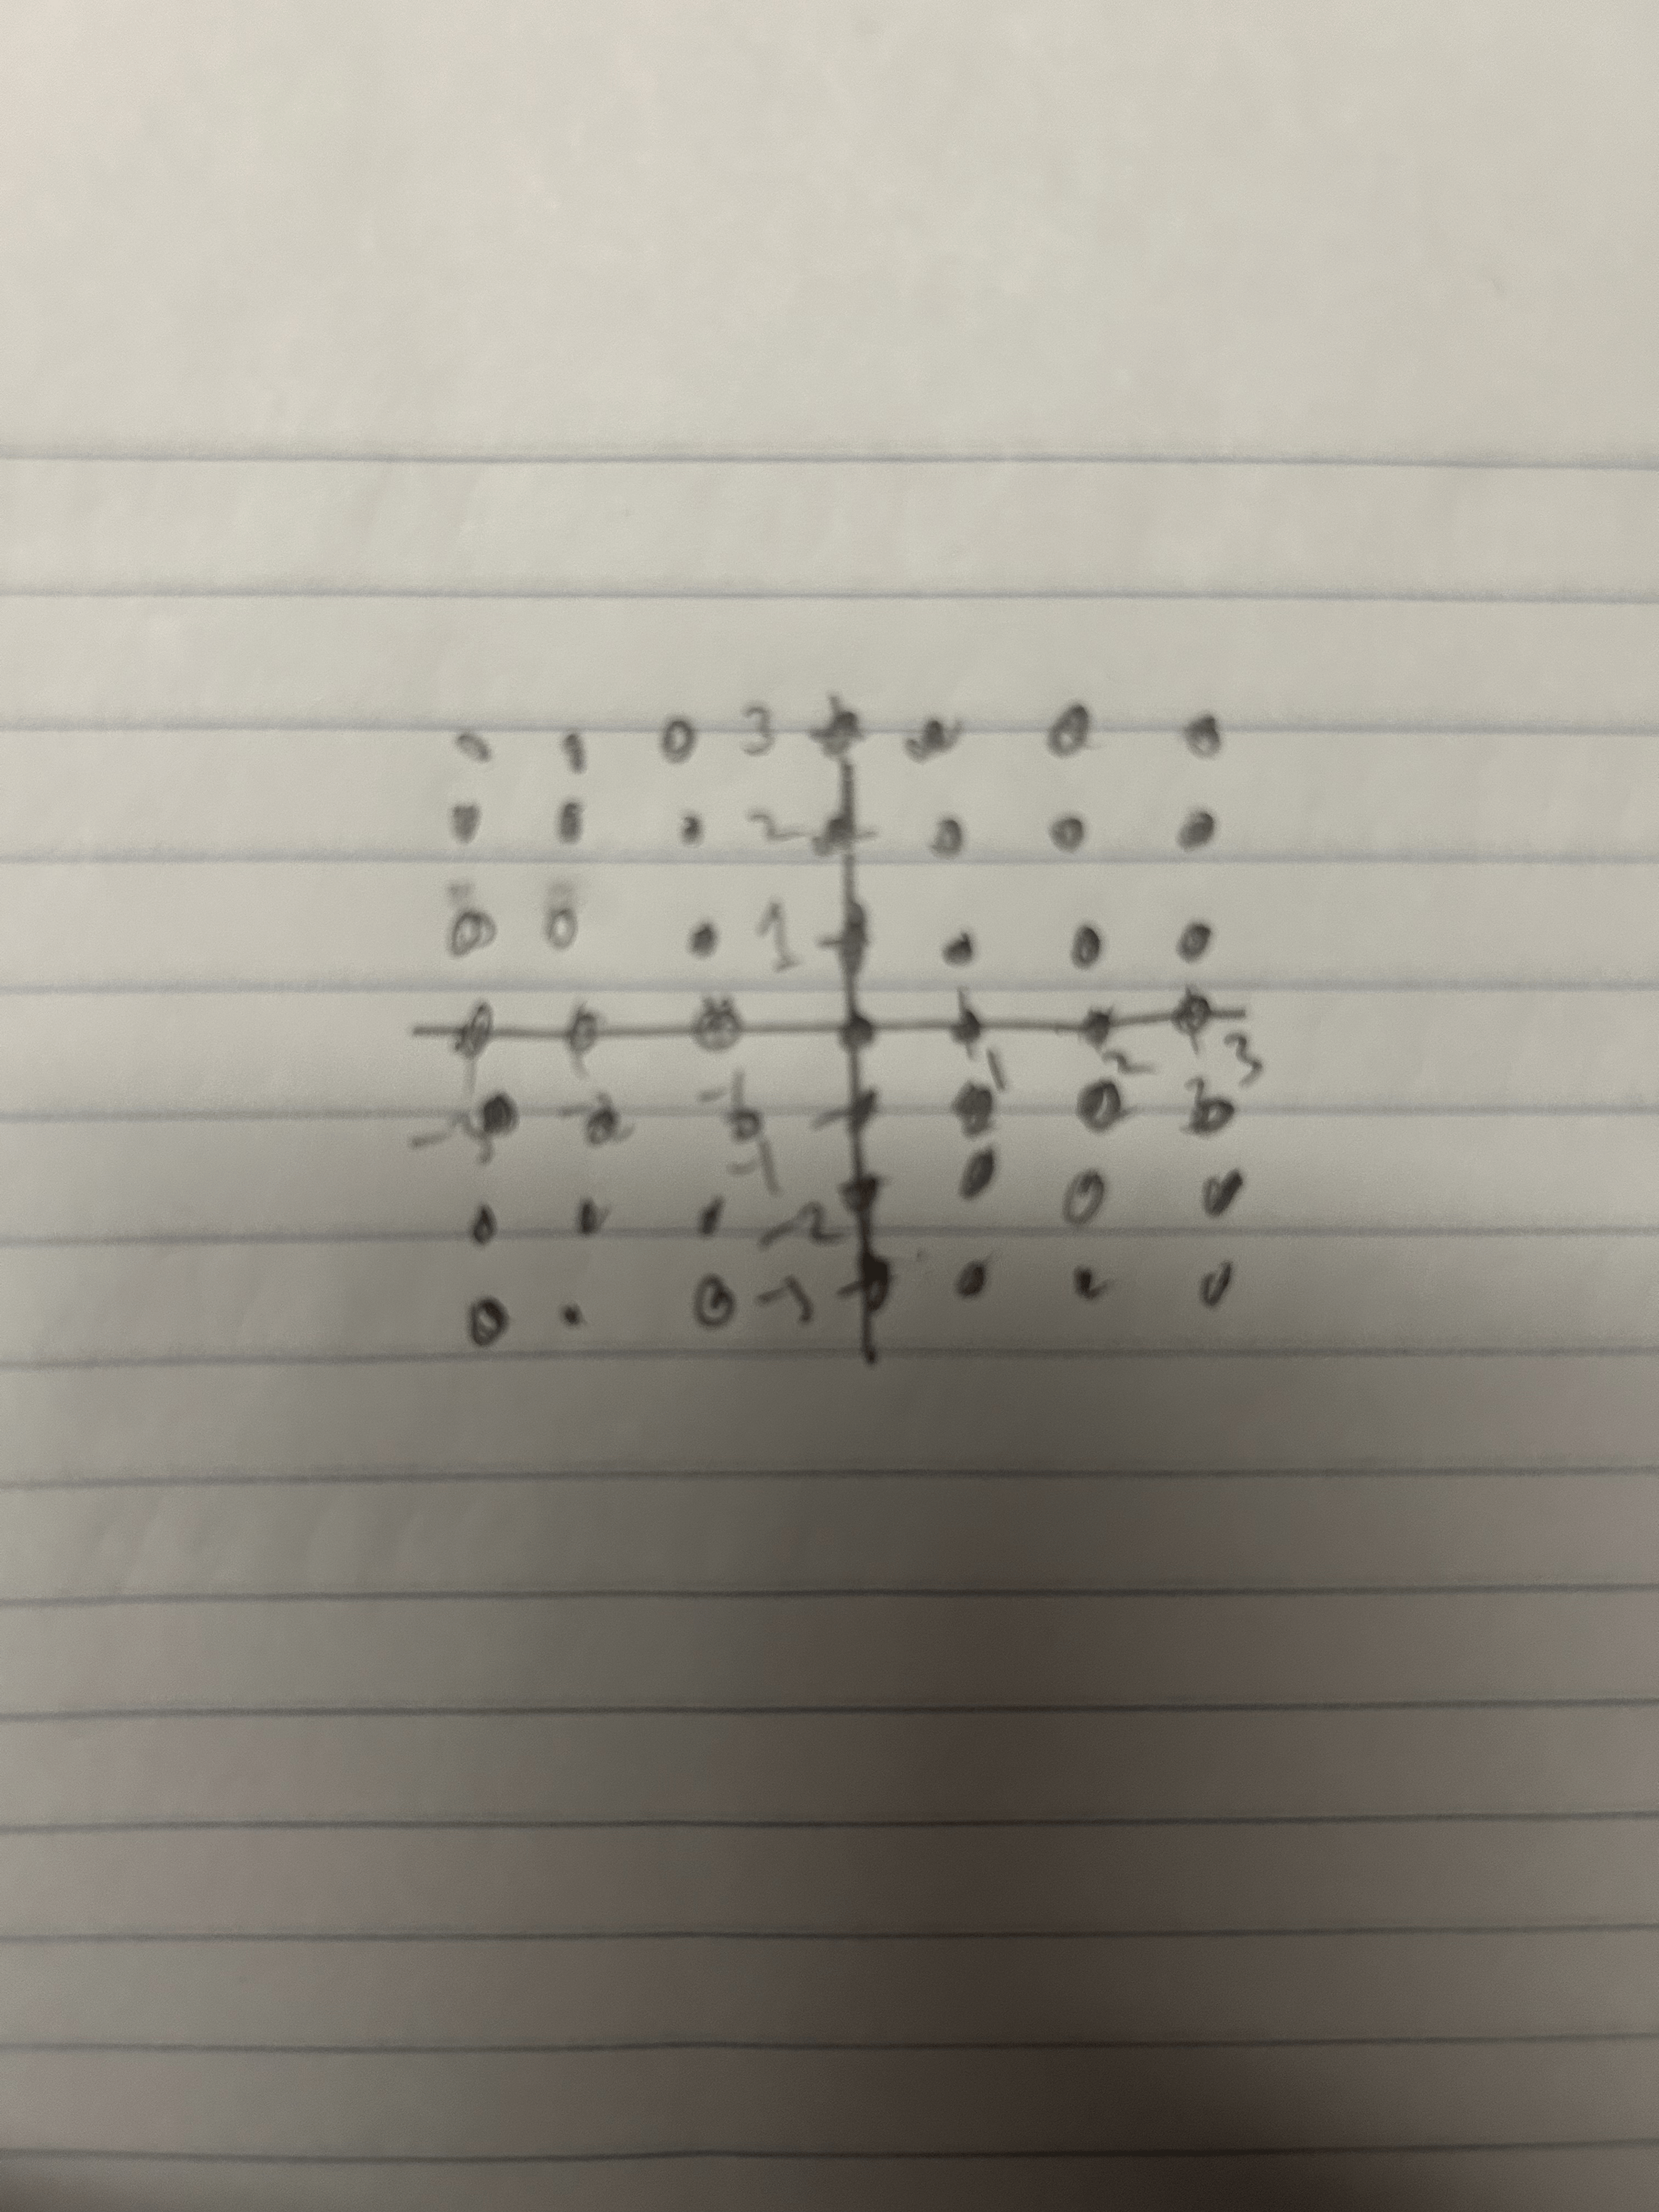
\includegraphics[width=0.3\textwidth]{IMG_1198}

\noindent \textbf{Chapter 1.4, Question 2:}
\begin{align*}
    \mathcal{P}(\set{1,2,3,4}) = \{ & \emptyset, \set{1}, \set{2}, \set{3}, \set{4},                    \\
                                    & \set{1,2}, \set{1,3}, \set{1,4}, \set{2,3}, \set{2,4}, \set{3,4}, \\
                                    & \set{1,2,3}, \set{1,2,4}, \set{1,3,4}, \set{2,3,4},               \\
                                    & \set{1,2,3,4} \}.
\end{align*}

\noindent \textbf{Chapter 1.4, Question 12:}
\begin{align*}
    \set{X \in \mathcal{P}(\set{1,2,3}) : 2 \in X} = \set{\set{2}, \set{1,2}, \set{2,3}, \set{1,2,3}}.
\end{align*}

\noindent \textbf{Chapter 1.4, Question 18:}

Suppose $|A| = m$ and $|B| = n$. Then,
\begin{align*}
    |\mathcal{P}(A \times \mathcal{P}(B))| & = 2^{|A| \cdot 2^{|B|}} \\
                                           & = 2^{m2^{n}}
\end{align*}

\noindent \textbf{Chapter 1.8, Question 10:}

(a)
\begin{align*}
    \bigcup_{x \in [0,1]}[x,1] \times [0, x^2] & = \set{(a,b) \in [0,1]^2 : b \leq a^2}.
\end{align*}

(b)
\begin{align*}
    \bigcap_{x \in [0,1]}[x,1] \times [0, x^2] & = \set{(1,0)}.
\end{align*}

\noindent \textbf{Chapter 3.5, Question 16:}

Suppose $A = \set{1,2, \ldots , 10}$.
Notice that $A$ has 5 even elements and 5 odd elements.
To have exactly 3 even elements in a 6-element subset means choosing 3 even and 3 odd.
That is, the number of 6-element subsets of $A$ with exactly 3 even elements is
\begin{equation*}
    \binom{5}{3}\binom{5}{3} = 100.
\end{equation*}

There are $\binom{10}{6}=210$ 6-element subsets of $A$.
So the number of them that don't have exactly 3 even elements is $210 - 100 = 110$.

\noindent \textbf{Chapter 3.10, Question 6:}

Let $n$ be a non-negative integer.
Consider $\binom{3n}{3}$.
This is the number of 3-element subsets of a set $S$ of size $3n$.
Partition $S$ into $A \cup B \cup C$, where $|A| = |B| = |C| = n$.

Every 3-element subset of $S$ falls into exactly 1 of these 3 cases:

Case A: All 3 elements are chosen from the same subset, either from $A$, $B$, or $C$.
So there are 3 options of subsets and $\binom{n}{3}$ ways to choose elements.
Thus, we have $3\binom{n}{3}$ distinct 3-element subsets.

Case B: We choose 2 elements from one subset and 1 element from another subset.
Then, there are $\binom{3}{1}$ ways to choose the subset with 2 elements,
$\binom{2}{1}$ ways to choose the other subset with 1 element,
and $\binom{n}{1}\binom{n}{2}$ ways to choose elements.
Thus, by multiplication principle, we have an additional $6n\binom{n}{2}$ distinct 3-element subsets.

Case C: We choose 1 element from each of the subsets.
That is, we have $\binom{n}{1}^3$ ways to choose the elements.
Thus, by multiplication principle, we have another $n^3$ distinct 3-element subsets.

Since all the cases are disjoint and completely cover all 3-element subsets,
it follows that we have a total of $3\binom{n}{3} + 6n\binom{n}{2} + n^3$ distinct 3-element subsets from $S$.

Both of these expressions count the same subsets of $S$. So we conclude
\begin{align*}
    \binom{3n}{3} = 3\binom{n}{3} + 6n\binom{n}{2} + n^3.
\end{align*}

\noindent \textbf{Chapter 8, Question 2:}

Let $A$ denote $\{ 6n : n \in{\mathbb{Z}} \}$, $B$ denote $\{ 2n : n \in{\mathbb{Z}} \}$, and $C$ denote $\{ 3n : n \in{\mathbb{Z}} \}$.

Suppose $a \in A$. That is, $a = 6k$ for some integer $k$.
Then,
\begin{align*}
    a & = 2(3k)                       \\
      & = 2w,  ~\text{where $w= 3k$.}
\end{align*}
Then, $w$ is an integer since it's the product of integers.
So $a \in B$.
We also have
\begin{align*}
    a & = 3(2k)                        \\
      & = 3z, ~ \text{where $z = 2k$.}
\end{align*}
Then, $z$ is an integer  since it's the product of integers.
So $a \in C$.
Since $a$ is in both $B$ and $C$, it follows that $a \in B \cap C$.
Thus, $A \subseteq B \cap C$.

Suppose $d \in B \cap C$.
That is, for some integers $x$ and $y$, we have $d = 2x$ and $d = 3y$.
Then, $2x = 3y$. So $3 \mid 2x$.
Since 3 is prime and $gcd(2, 3) = 1$, by Euclid's Lemma, we have $ 3 \mid x$.
That is, for some integer $n$, $x = 3n$.
Then,
\begin{align*}
    d & = 2(3n) \\
      & = 6n.
\end{align*}
So $d \in A$.
Thus, $B \cap C \subseteq A$.

Since $A \subseteq B \cap C$ and $B \cap C \subseteq A$, we conclude $A = B \cap C$. That is,
\begin{align*}
    \{6n : n \in{\mathbb{Z}} \} = \{ 2n : n \in{\mathbb{Z}} \} \cap \{ 3n : n \in{\mathbb{Z}} \}.
\end{align*}

\noindent \textbf{Chapter 8, Question 16:}

Let $A$, $B$, and $C$ be sets.

Let $x \in A$ and $y \in B \cup C$.
Then, $(x,y) \in A \times (B \cup C)$.
Since $y$ is either in $B$ or $C$, we have 2 cases for $y$.

\noindent{}Case 1: $y \in B$.
So $(x,y) \in A \times B$.

\noindent{}Case 2: $y \in C$.
So $(x,y) \in A \times C$.

\noindent{}Thus, $(x,y) \in (A \times B) \cup (A \times C)$.
Then, $A \times (B \cup C) \subseteq (A \times B) \cup (A \times C)$.

Let $(a, d) \in (A \times B) \cup (A \times C)$.
Then, we have the following 2 cases:

\noindent{}Case 1: $(a, d) \in (A \times B)$.
So $a \in A$ and $d \in B$.

\noindent{}Case 2: $(a, d) \in (A \times C)$.
So $a \in A$ and $d \in C$.

\noindent{}Notice that $a$ is always in $A$, while $d$ is either in $B$ or $C$.
That is, $a \in A$ and $d \in B \cup C$.
So $(a, d) \in A \times (B \cup C)$.
Thus, $(A \times B) \cup (A \times C) \subseteq A \times (B \cup C)$.

Therefore, $(A \times B) \cup (A \times C) = A \times (B \cup C)$.

\noindent \textbf{Chapter 8, Question 28:}

Let $X$ denote $\{12a + 25b: a,b \in \mathbb{Z}\}$.

Suppose $x \in X$.
Then, $x = 12a + 25b$ for some integers $a$ and $b$.
Since $x$ is a sum of products of integers, $x$ is an integer.
So $x \in \mathbb{Z}$.
Thus, $X \subseteq \mathbb{Z}$.

Suppose $z \in \mathbb{Z}$.
Consider $12a + 25b$.
Let $a = -2z$ and $b = z$.
Since $z$ is an integer, $a$ and $b$ are also integers.
Then,
\begin{align*}
    12(-2z) + 25(z) = z.
\end{align*}
Thus, we have found $a$ and $b$ such that $12a + 25b = z$.
So, $z \in X$.
Thus, $\mathbb{Z} \subseteq X$.

Since we have $X \subseteq \mathbb{Z}$ and $\mathbb{Z} \subseteq X$, we can conclude that $X = \mathbb{Z}$.
That is,
\begin{align*}
    \{12a + 25b: a,b \in \mathbb{Z}\} = \mathbb{Z}.
\end{align*}


\end{document}

